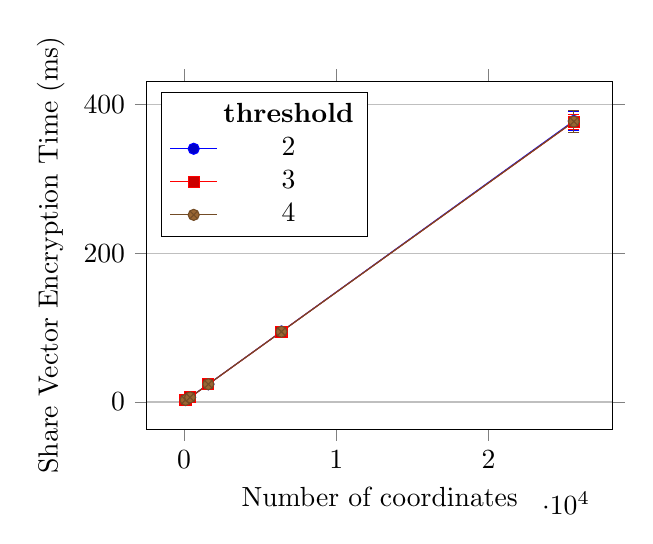
\begin{tikzpicture}
\begin{axis}[
    width=7.5cm,
    height=6cm,
    %xmode=log,
    %log basis x=10,
    xlabel={Number of coordinates},
    ylabel={Share Vector Encryption Time (ms)},
    yticklabel style={
    /pgf/number format=float,
    /pgf/number format/precision=2
    },
    scaled y ticks=false,
    scaled y ticks=false,
    legend pos=north west,
    tick align=outside,
    grid=both,
    xmajorgrids=false,
]

% Fake legend title
\addlegendimage{empty legend}
\addlegendentry{\textbf{threshold}}

% Threshold 2
\addplot+[error bars/.cd,
        y dir=both,
        y explicit] coordinates {
    (100,2.77553) +- (0,0.250630359)
    (400,6.31184) +- (0,0.3847697664)
    (1600,24.0407) +- (0,1.1155816)
    (6400,94.9017) +- (0,2.25866046)
    (25600,378.331) +- (0,12.939525529)
};
\addlegendentry{2}

% Threshold 3
\addplot+[error bars/.cd,
        y dir=both,
        y explicit] coordinates {
    (100,2.7739) +- (0,0.232276954)
    (400,6.29326) +- (0,0.25499236)
    (1600,23.8682) +- (0,0.98098302)
    (6400,94.7617) +- (0,6.68691621752)
    (25600,377.202) +- (0,10.096188732)
};
\addlegendentry{3}

% Threshold 4
\addplot+[error bars/.cd,
        y dir=both,
        y explicit] coordinates {
    (100,2.84632) +- (0,0.1908451)
    (400,6.30467) +- (0,0.556056762)
    (1600,23.9751) +- (0,2.0936101)
    (6400,94.652) +- (0,5.5189498856)
    (25600,377.374) +- (0,15.21775749)
};
\addlegendentry{4}

\end{axis}
\end{tikzpicture}